\section{Auswertung}
\subsection{Fouriersynthese}
\begin{figure}[h]
\begin{subfigure}{0.5\textwidth}
    \centering
    \includegraphics[width=\textwidth]{assets/rechteck_oszi.jpg}
    \caption{Rechteckschwingung}
\end{subfigure}
\begin{subfigure}{0.5\textwidth}
    \centering
    \includegraphics[width=\textwidth]{assets/dreieck_oszi.jpg}
    \caption{Dreieckschwingung}
\end{subfigure}
\begin{subfigure}{0.5\textwidth}
    \centering
    \includegraphics[width=\textwidth]{assets/zahn_oszi.jpg}
    \caption{Sägezahnschwingung}
\end{subfigure}
\caption{Mit dem Oszilloskop aufgezeichnete Schwingungsbilder}
\label{fig:oszi}
\end{figure}

In Abbildung \ref{fig:oszi} sind die aufgezeichneten Schwingungsbilder für die drei eingestellten Schwingungen dargestellt. Es zeigt sich, dass alle drei in guter Übereinstimmung mit den in der Vorbereitung vorhergesagten Kurven stehen.
\newpage
\subsection{Fourieranalyse}
\begin{table}[h]
	\centering
	\caption{Aufgenommene Messwerte zur Rechteckspannung}
	\label{tab:rechteck_messwerte}
	\begin{tabular}{ S S S S }
		\toprule
		{ $\text{Oberschwingung} \: n $ } & { $ \nu \: / \: \si{kHz} $} & {$ \text{Amplitude} \: / \: \si{dB} $} & {$ \text{Amplitude}\: U \: / \: \si{V} $}\\
		\midrule
            1 & 100 & 39.0 & 89.12 \\ 
            3 & 300 & 29.4 & 29.51 \\
            5 & 500 & 25.0 & 17.78 \\
            7 & 700 & 22.2 & 12.88 \\
            9 & 900 & 20.6 & 10.71 \\
            11 & 1100 & 19.0 & 8.91 \\
            13 & 1300 & 17.8 & 7.76 \\
            15 & 1500 & 16.6 & 6.76 \\
            17 & 1700 & 16.2 & 6.45 \\
            19 & 1900 & 15.4 & 5.88 \\
	\end{tabular}
\end{table}

\begin{table}[h]
	\centering
	\caption{Aufgenommene Messwerte zur Dreieckspannung}
	\label{tab:dreieck_messwerte}
	\begin{tabular}{ S S S S }
		\toprule
		{ $\text{Oberschwingung} \: n $ } & { $ \nu \: / \: \si{kHz} $} & {$ \text{Amplitude} \: / \: \si{dB} $} & {$ \text{Amplitude}\: U \: / \: \si{V} $}\\
		\midrule
            1 & 100 & 35.00 & 56.23 \\ 
            3 & 300 & 16.20 & 6.46 \\
            5 & 500 & 7.01 & 2.241 \\
            7 & 700 & 1.81 & 1.23 \\
            9 & 900 & -2.99 & 0.71 \\
            11 & 1100 & -6.59 & 0.47 \\
            13 & 1300 & -8.59 & 0.37 \\
	\end{tabular}
\end{table}

\begin{table}[h]
	\centering
	\caption{Aufgenommene Messwerte zur Sägezahnspannung}
	\label{tab:zahn_messwerte}
	\begin{tabular}{ S S S S }
		\toprule
		{ $\text{Oberschwingung}\: n $ } & { $ \nu \: / \: \si{kHz} $} & {$ \text{Amplitude} \: / \: \si{dB} $} & {$ \text{Amplitude}\: U \: / \: \si{V} $}\\
		\midrule
            1 & 100 & 32.8 & 43.65 \\ 
            2 & 205 & 27.0 & 22.38 \\
            3 & 305 & 22.6 & 13.49 \\
            4 & 405 & 21.4 & 11.75 \\
            5 & 505 & 19.8 & 9.77 \\
            6 & 605 & 18.2 & 8.13 \\
            7 & 705 & 17.4 & 7.41 \\
            8 & 810 & 16.6 & 6.76 \\
            9 & 910 & 15.8 & 6.16 \\
            10 & 1010 & 15.4 & 5.89 \\
	\end{tabular}
\end{table}
In den Tabellen \ref{tab:rechteck_messwerte} bis \ref{tab:zahn_messwerte} sind die vom Oszilloskop abgelesenen Positionen und Höhen der Peaks der jeweiligen Schwingungen aufgelistet. Es is zu beobachten, dass sowohl bei der Rechteck- als auch bei der Dreieckschwingung keine Peaks für gerade $n$ ablesen lassen. Dies steht in Übereinstimmung mit den in der Vorbereitung gemachten Vorhersagen. In den Abbildungen \ref{fig:rechteck_fit} bis \ref{fig:zahn_fit} sind die Höhen der Peaks einmal gegen die Frequenz und einmal doppelt logarithmisch gegen $n$ aufgetragen. Da sich für alle drei Schwingungsformen die Fourierkoeffizienten aus einer Gleichung der Form
\begin{equation*}
    a_n = \frac{C}{n^k} = C \cdot n^{-k}
\end{equation*}
ergeben, können diese durch logarithmieren in eine Geradengleichung der Form
\begin{equation*}
    \log{a_n} = -k \cdot \log{n} + \log{C}
\end{equation*}
gebracht werden. Aus der Steigung der Geraden kann dann direkt der Exponent abgelesen werden.
Die jeweiligen Parameter für die Geradengleichung wurden mit der polyfit-Funktion von Python bestimmt zu
\begin{align*}
    -k = \num{0.923 \pm 0.019}
    \log{C} = \num{4.420 \pm 0.043}
\end{align*}
für die Rechteckschwingung, 
\begin{align*}
    -k = \num{1.976 \pm 0.018}
    \log{C} = \num{4.024 \pm 0.035}
\end{align*}
für die Dreieckschwingung und 
\begin{align*}
    -k = \num{0.867 \pm 0.031}
    \log{C} = \num{3.693 \pm 0.051}
\end{align*}
bestimmt.

\begin{figure}[h]
\begin{subfigure}{0.5\textwidth}
    \centering
    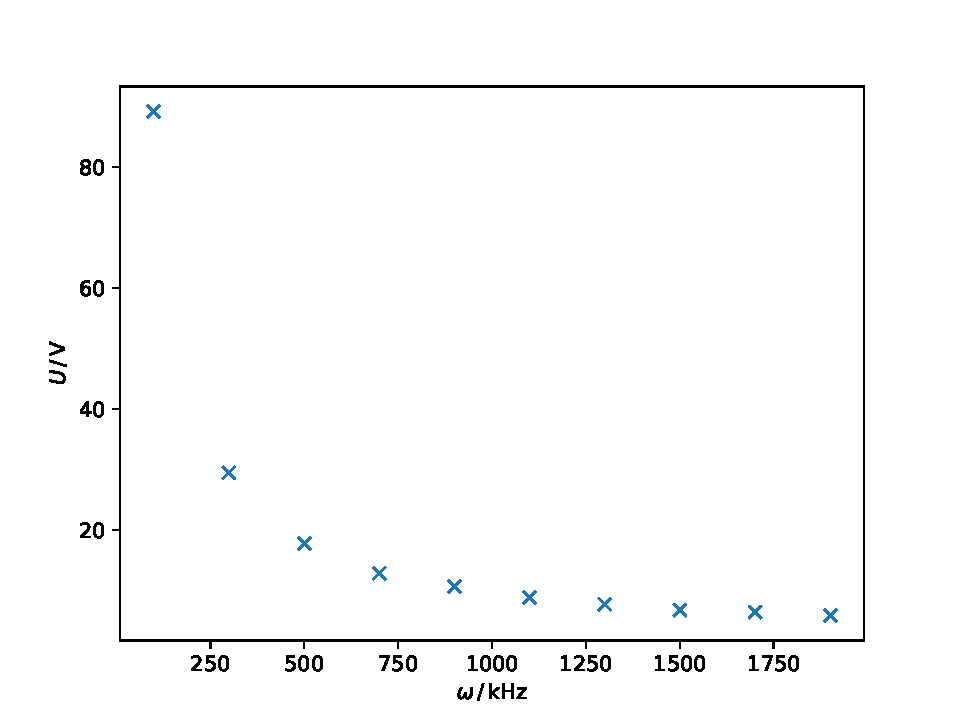
\includegraphics[width=\textwidth]{assets/rechteck_messung.pdf}
\end{subfigure}
\begin{subfigure}{0.5\textwidth}
    \centering
    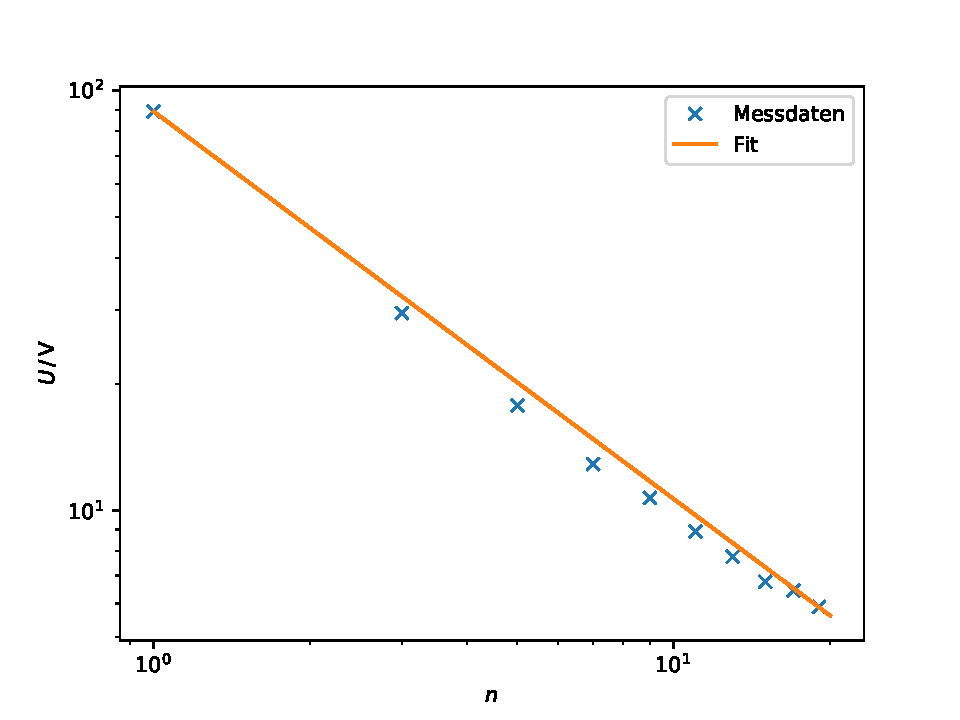
\includegraphics[width=\textwidth]{assets/rechteck_log.pdf}
\end{subfigure}
\caption{Messdaten für die Rechteckschwingung}
\label{fig:rechteck_fit}
\end{figure}

\begin{figure}[h]
\begin{subfigure}{0.5\textwidth}
    \centering
    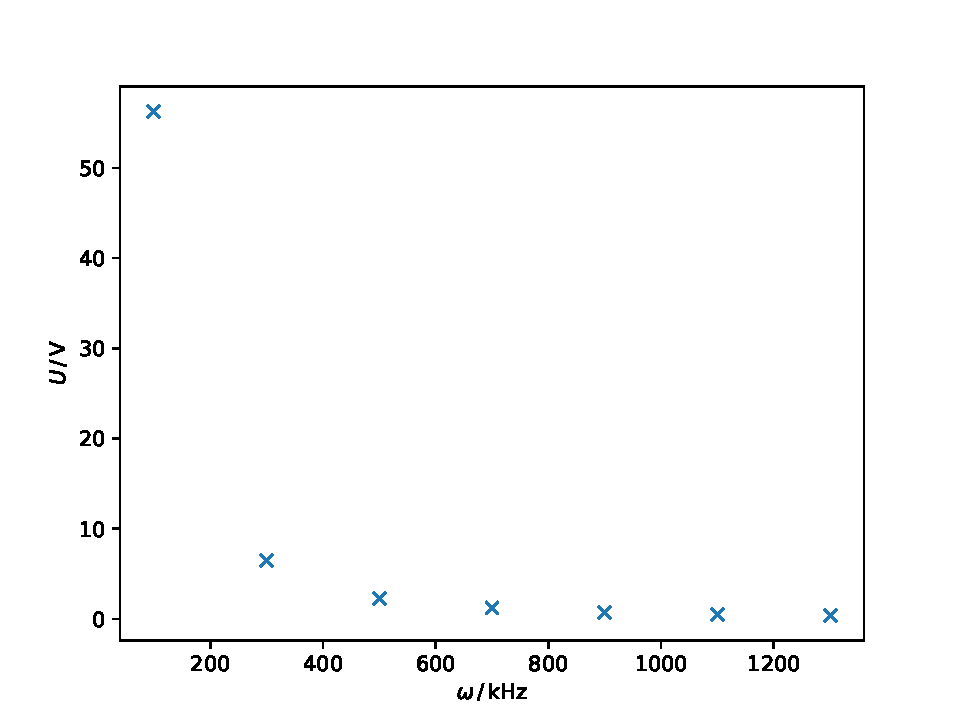
\includegraphics[width=\textwidth]{assets/dreieck_messung.pdf}
\end{subfigure}
\begin{subfigure}{0.5\textwidth}
    \centering
    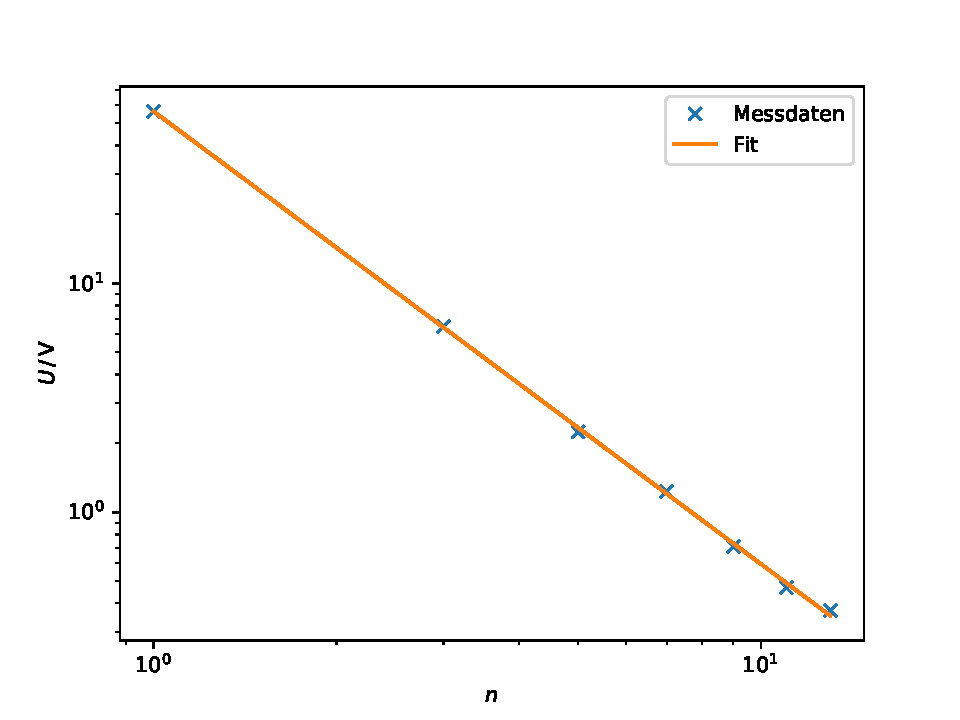
\includegraphics[width=\textwidth]{assets/dreieck_log.pdf}
\end{subfigure}
\caption{Messdaten für die Dreieckschwingung}
\label{fig:dreieck_fit}
\end{figure}



\begin{figure}[h]
\begin{subfigure}{0.5\textwidth}
    \centering
    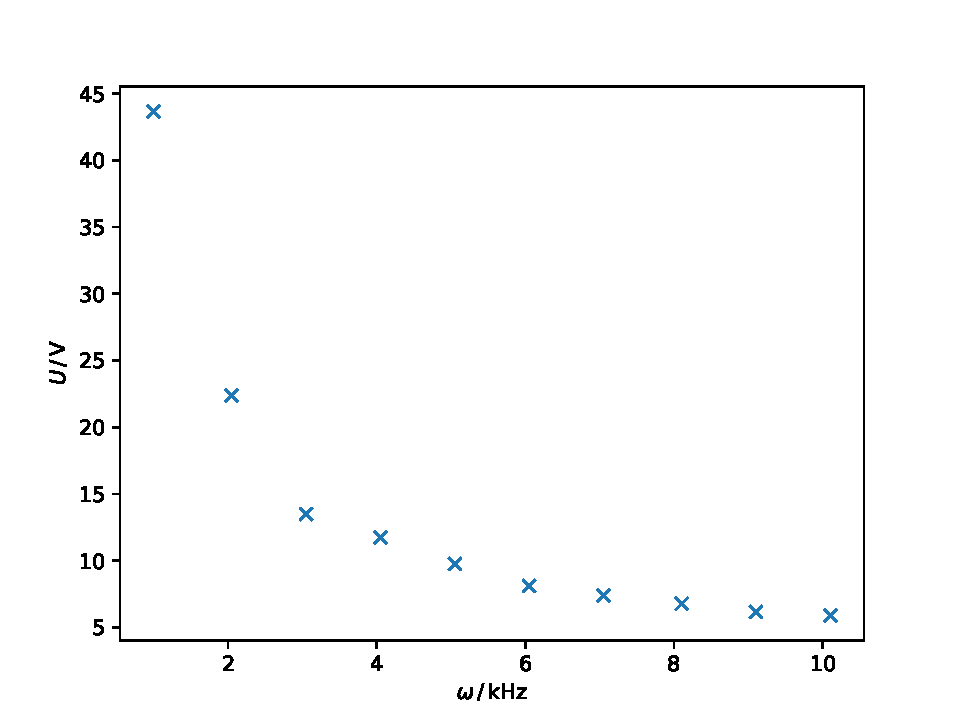
\includegraphics[width=\textwidth]{assets/zahn_messung.pdf}
\end{subfigure}
\begin{subfigure}{0.5\textwidth}
    \centering
    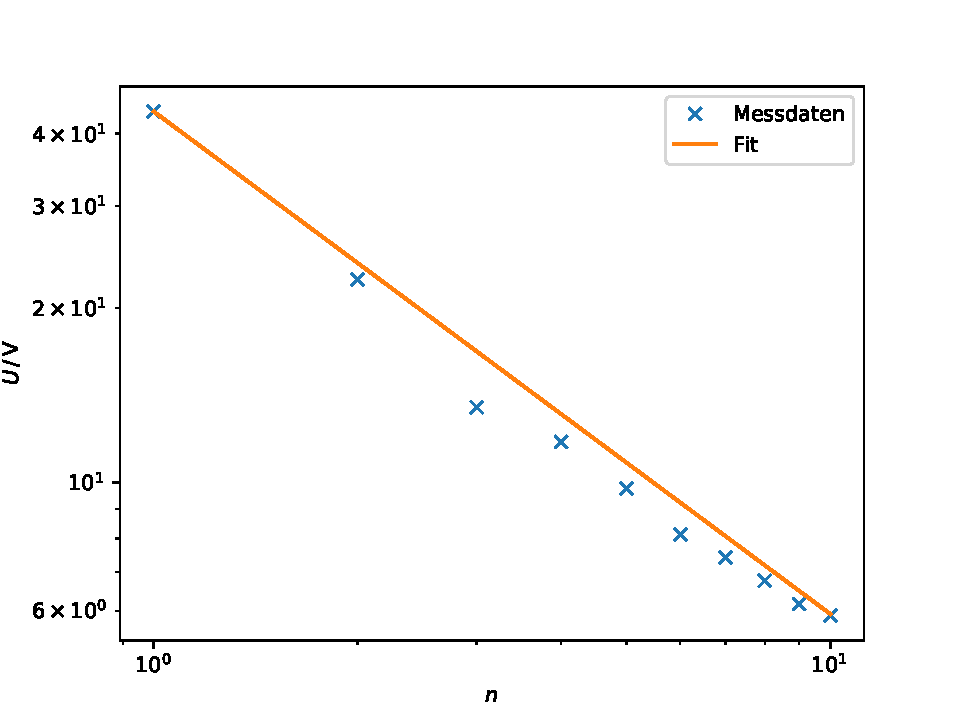
\includegraphics[width=\textwidth]{assets/zahn_log.pdf}
\end{subfigure}
\caption{Messdaten für die Sägezahnschwingung}
\label{fig:zahn_fit}
\end{figure}
